\chapter{Dasar Teori}
\label{chap:dasar teori}

Sebelum bisa membuat Twitter bot untuk mencari jalur transportasi publik, berikut diberikan beberapa definisi yang berkaitan dengan pembuatan Twitter bot. Bab ini akan menjelaskan Twitter, Twitter API, KIRI, KIRI API, dan Twitter4j.

\section{Twitter}
\label{sec:twitter}

Twitter adalah layanan yang memungkinkan pengguna untuk mengirim pesan menggunakan 140 karakter atau kurang. Pesan tersebut dapat diadaptasikan melalui teks, aplikasi \textit{mobile}, atau web. (referensi dari buku Sams teach yourself the twitter api) Berikut ini adalah daftar istilah umum pada Twitter:

Twitter adalah salah satu layanan jejaring sosial online yang memungkinkan pengguna melakukan \textit{posting} pesan berbasis teks hingga 140 karakter\cite{TwitterBook}.
\begin{itemize}
	\item \textit{Tweet} 
	
	Posting pada Twitter disebut sebagai \textit{tweet}. \textit{Tweet} ini akan meneruskan pesan singkat yang ditujukan ke semua \textit{follower} suatu akun\footnote{Dusty Reagan, \textit{Twitter Application Development For Dummies}, Wiley, 2010, page 7}. Contohnya adalah seorang akun @kviniink ingin menuliskan bahwa hari ini cuaca cerah, maka @kviniink akan men-\textit{tweet} 'Hari ini cerah yah..'. \textit{Tweet} juga bisa menyertakan \textit{link} ke video, foto, atau media lain di internet selain teks biasa. URL \textit{link} teks termasuk ke dalam 140 batas karakter, namun URL tersebut akan menghabisnya tempat/\textit{space} dari keterbatasan karakter tweet. Oleh karena itu URL akan dibuat versi singkatnya, contoh saat pengguna memasukkan link \url{http://www.chacha.com/gallery/7253/15-movies-that-make-guys-cry}, maka akan dibuat menjadi \url{bit.ly/1uRi8vV}. 
	\item \textit{Follow}
	
	\textit{Follow} adalah satu istilah dalam Twitter yang bertujuan untuk mengikuti aktivitas \textit{tweet} suatu akun. \textit{Following} adalah ketika sebuah akun mengikuti akun orang lain, dan \textit{Follower} adalah ketika sebuah akun melakukan aksi \textit{follow} kepada akun anda.
	\item \textit{Reply} 
	
	\textit{Reply} adalah cara seseorang untuk dapat memberi rujukan kepada akun Twitter yang lainnya atau lebih dikenal dengan nama \textit{mention}\footnote{Dusty Reagan, \textit{Twitter Application Development For Dummies}, Wiley, 2010, page 9}. Sebagai contoh, diketahui akun bernama @kviniink mem-\textit{follow} @infobdg untuk mengetahui perkembangan apa saja yang tejadi di Kota Bandung. Lalu akun @kviniink ingin bertanya tentang info mall yang ramai di Kota Bandung, maka akun @kviniink membuat \textit{mention tweet} yang berisikan "@infobdg Halo saya ingin bertanya apa saja mall yang sedang ramai di Bandung yah?".
	\item \textit{Retweet}
	
	\textit{Retweet} ini merupakan salah satu yang paling penting dari Twitter. \textit{Retweet} ini berguna ketika pengguna menemukan \textit{tweet} menarik dan berbagi \textit{tweet} tersebut dengan \textit{follower} akun tersebut (\textit{follower}). \textit{Retweet} ini juga secara tidak langsung mengatakan bahwa "saya menghormati anda dan pesan yang anda buat". \textit{Retweet}.
	%\footnote{Tim O’Reilly, \textit{The Twitter Book}, oreilly, 2009, page 47}
	\item \textit{Hashtag}
	
	Sebuah fitur yang diciptakan oleh Twitter untuk membantu pencarian kata kunci dan penandaan suatu diskusi.
	
	\item \textit{Direct Message}(DM)
	
	\textit{Direct message} digunakan untuk mengirim pesan yang bersifat \textit{private} antara dua orang. Orang yang mengirim \textit{direct message} ini hanya bisa untuk orang yang mengikuti akun tersebut.
	\item \textit{Timeline}
	
	\textit{Timeline} adalah sekumpulan \textit{tweet} dari semua orang yang anda \textit{follow} lalu akan ditampilkan di halaman utama.
\end{itemize}


\section{Twitter API}
Twitter API adalah aplikasi pihak ketiga yang memungkinkan \textit{programmer} melakukan manipulasi dan pengolahan data di Twitter. Twitter API tidak seperti API pada umumnya karena Twitter memaparkan hampir semuanya termasuk \textit{setup account} dan informasi kostumisasi\cite{Twitter}. Ini adalah salah satu bentuk pendekatan dari Twitter yang berfokus pada jaringan dan memungkinkan developer memiliki hak untuk berpikir '\textit{out of the box}' untuk membuat aplikasi yang mereka inginkan. Tetapi tetap akan terjadi keterbatasan yang dimiliki Twitter API, yaitu :
\begin{itemize}
	\item Hanya bisa men-update 1000 per harinya, baik melalui handphone, website, API, dan sebagainya.
	\item Total pesan hanya bisa sebanyak 250 per harinya, pada setiap dan semua perangkat.
	\item 150 permintaan API per jam.
	\item OAuth diijinkan 350 permintaan per jam.
\end{itemize}

\subsection{\textit{Search} API}

Twitter \textit{Search} API memungkinkan melakukan pencarian terhadap \textit{tweet} baru ataupun \textit{tweet} populer. Tetapi Twitter \textit{Search} API ini bukan fitur yang tersedia pada Twitter itu sendiri. API ini difokuskan kepada relefansi, bukan terhadap kelengkapan data. Ini berarti bahwa beberapa \textit{Tweet} dan pengguna akan hilang dari hasil pencarian.

\paragraph{Bagaimana cara membuat sebuah \textit{query}}
Cara berbaik dalam membuat sebuah \textit{query}, melakukan percobaan yang valid dan mengembalikan tweet yang sesuai adalah dengan mencobanya di \url{twitter.com/search}. URL yang ditampilkan pada browser akan berisi sintaks \textit{query} yang sesuai agar dapat digunakan kempali pada API \textit{endpoint}. Berikut adalah contohnya:

\begin{enumerate}
	\item Melakukan pencarian untuk \textit{tweet} yang direferensikan kepada akun @twitterapi. Pertama kita harus melakukan pencarian pada \url{twitter.com/search}.
	\item Lakukan pengecekan dan salin URL yang ditampilkan. Sebagai contoh didapatkan URL seperti ini, \url{https://twitter.com/search?q=\%40twitterapi}.
	\item Ganti "\url{https://twitter.com/search}" dengan "\url{https://api.twitter.com/1.1/search/tweets.json}" dan akan didapatkan "\url{https://api.twitter.com/1.1/search/tweets.json?q=\%40twitterapi}"
	\item Eksekusi URL tersebut untuk melakukan pencarian di dalam API.
\end{enumerate}

API v1.1 mewajibkan bahwa \textit{request} sudah diotentifikasi. Perlu diingat juga bahwa hasil pencarian yang dilakukan di \url{twitter.com} dapat menghasilkan hasil yang sudah sangat lama, sedangkan Search API hanya melayani tweet dari seminggu terakhir.

\begin{table}[h]
\caption{Contoh berbagai macam pencarian \textit{tweet}}
\begin{tabular}{|l|l|}
\hline
\textbf{Operator}          					& \textbf{Finds \textit{tweets}}                                            \\ \hline
\textit{watching now}               & Mengandung kata "\textit{watching}" dan "\textit{now}". 						       \\
"\textit{happy hour}"               & Mengandung frase "\textit{happy hour}" yang tepat.                                 \\
\textit{love OR hate}               & Mengandung kata "\textit{love}" atau "\textit{hate}" (atau keduanya).                             \\
\textit{beer -root}                 & Mengandung kata "\textit{beer}" tanpa kata "\textit{root}".                                         \\
\#haiku                    					& Mengandung \textit{hashtag} "\textit{haiku}".                                            \\
\textit{from}:alexiskold            & Dikirim melalui \textit{user} "alexiskold".                                            \\
\textit{to}:techcrunch              & Dikirimkan kepada \textit{user} "techcrunch".                                              \\
@mashable                  					& Mereferensikan kepada \textit{user} "mashable".                                            \\
\textit{superhero since}:2010-12-27 & Mengandung kata "\textit{superhero}" dari tanggal "2010-12-27" (tahun-bulan-hari). \\
\textit{ftw until}:2010-12-27       & Mengandung kata "\textit{ftw}" sebelum tanggal "2010-12-27".                   \\
\textit{movie -scary} :)            & Mengandung kata "\textit{movie}", tanpa kata "\textit{scary}", dengan pencarian yang positif.        \\
\textit{flight} :(                  & Mengandung kata "\textit{flight}" dengan pencarian yang negatif.                         \\
\textit{traffic} ?                  & Mengandung kata "\textit{traffic}" dan mengandung pertanyaan.                               \\
\textit{hilarious filter:links}     & Mengandung kata "\textit{hilarious}" yang di sambungkan dengan URL.                                \\
\textit{news source:twitterfeed}    & Mengandung kata "\textit{news}" yang dipost melalui twitterfeed.						\\        \hline                     
\end{tabular}
\end{table}

Dipastikan bahwa pengkodean URL terhadap \textit{query} dilakukan terlebih dahulu sebelum melakukan \textit{request}. Tabel berikut memberikan contoh \textit{mapping} dari \textit{search quer}y ke \textit{query} pengkodean URL.

\begin{table}[h]
\begin{tabular}{|l|l|}
\hline
\textbf{\textit{Search query}}     & \textbf{\textit{URL encoded query}}                 \\ \hline
\#haiku \#poetry & \%23haiku+\%23poetry              \\
"\textit{happy hour}" :)  & \%22\textit{happy}\%20\textit{hour}\%22\%20\%3A\%29 \\ \hline
\end{tabular}
\end{table}

\paragraph{\textit{Additional parameters}}
Terdapat parameter tambahan yang dipergunakan untuk hasil pencarian yang lebih baik. Berikut adalah penjelasan dari parameter tambahan tersebut :

\begin{itemize}
	\item \textbf{\textit{Result Type}}. Seperti hasil yang terdapat pada \url{twitter.com/search}, parameter \textit{result\_type} memungkinkan hasil pencarian akan berdasarkan \textit{tweet} yang paling baru atau \textit{tweet} yang paling poluler atau bahkan gabungan dari keduanya.
	\item \textit{\textbf{Geolocatization}}. Pencarian tempat tidak tersedia pada API, tetapi ada beberapa cara yang tepat untuk membatasi \textit{query} dengan cara menggunakan parameter geocode lalu menentukan "\textit{latitude, longitude, radius}". Contohnya adalah "37.781157,-122.398720,1mi". Ketika pencarian lokasi pencarian API pertama akan mencoba menemukan \textit{tweet} yang memiliki \textit{latitude} yang sudah dimasukan kedalam \textit{query} geocode, jika tidak berhasil maka API akan mencoba menemukan \textit{tweet} yang dibuat oleh pengguna yang lokasi profilenya terdapat pada \textit{latitude} tersebut. Artinya adalah hasil pencarian mungkin menerima \textit{tweet} yang tidak mencakup informasi \textit{latidute} atau \textit{longitude}.
	\item \textit{\textbf{Language}}. Bahasa dapat dijadikan parameter untuk mencari tweet yang sesuai dengan bahasa tersebut.
	\item \textbf{\textit{Iterating in a result set}}. Parameter seperti \textit{count, until, since\_id, max\_id} memungkinkan untuk mengkontrol bagaimana iterasi melalui hasil pencarian.
\end{itemize}

\paragraph{\textit{Rate limits}}
\textit{User} pada saat ini diwakilkan oleh \textit{access tokens} yang dapat membuat 180 \textit{request} per 15 menit. Tetapi kita bisa membuat 450 \textit{request} per 15 menit dengan cara menggunakan \textit{application-only authentication} atas nama sendiri tanpa konteks pengguna.

\paragraph{Contoh Pencarian}
Ketika anda mengikuti suatu acara yang sedang berlangsung, anda tertarik untuk mencarinya dengan melihat tweet yang paling baru dan menggunakan \textit{hastag} dari acara tersebut, maka langkah-langkah yang dilakukan adalah:
\begin{itemize}
	\item Anda ingin mencari \textit{tweet} yang paling baru dengan menggunakan hastag \#\textit{superbowl}
	\item Maka \textit{search} URL akan seperti ini:
	\url{https://api.twitter.com/1.1/search/tweets.json?q=\%23superbowl\&result\_type=recent}
\end{itemize}

Ketika anda ingin mengetahui \textit{tweet} yang datang dari suatu lokasi dengan bahasa yang spesifik, maka langkah-langkah yang dilakukan adalah:
\begin{itemize}
	\item Anda ingin mencari \textit{tweet} yang paling baru dalam Bahasa Portugal, yang lokasinya dekat Maracanã soccer stadium yang terletak di Rio de Janeiro.
	\item Maka search URL akan seperti ini:
	\vtop{\hbox{\strut \url{https://api.twitter.com/1.1/search/tweets.json?}\hbox{\strut q=\&geocode=-22.912214,-43.230182,1km\&lang=pt\&result\_type=recent}}}
	%%%https://api.twitter.com/1.1/search/tweets.json?q=\&geocode=-22.912214,-43.230182,1km\&lang=pt\&result\_type=recent
	
Ketika anda ingin mencari \textit{tweet} yang sedang poluler dari spesifik \textit{user} dan \textit{tweet} tersebut terdapat sebuah hashtag tertentu:
\begin{itemize}
	\item Anda ingin mencari \textit{tweet} yang poluler yang berasal dari \textit{user} @kviniink yang terdapat \textit{hashtag} \#nasa.
	\item Maka \textit{search} URL akan seperti ini:
	\url{https://api.twitter.com/1.1/search/tweets.json?q=from\%3Akviniink\%20\%23nasa\&result\_type=popular}
\end{itemize}
\end{itemize}

\subsection{Streaming API}
\textit{Streaming} API adalah contoh \textit{real-time} API. API ini ditujukan bagi para pengembang dengan kebutuhan data yang intensif. Contohnya jika mencari cara untuk membangun sebuah data produk \textit{data-mining} atau tertarik dalam analisis penelitian. \textit{Streaming} API memungkinkan melacak kata kunci yang ditentukan dalam jumlah besar dan melakukan suatu aksi (seperti \textit{tweet}) secara langsung atau \textit{real-time}.

Twitter menawarkan beberapa \textit{endpoint streaming}, disesuaikan dengan kasus yang terjadi. 
\begin{itemize}
	\item \textit{Public stream}
	
	\textit{Steaming} data publik yang mengalir melalui Twitter. Dipergunakan untuk mengikuti sebuah \textit{user} atau topik tertentu. Selain itu juga \textit{public stream} digunakan untuk \textit{data mining}.
	\item \textit{User Stream}
	
	\textit{Single-user streams}, mengandung hampir semua data yang berhubungan dengan satu \textit{user} tertentu.
	
	\item \textit{Site Stream}
	
	Versi dari \textit{multi-user stream}. \textit{Site stream} harus terhubung dengan server yang terkoneksi dengan Twitter atas nama banyak pengguna.
\end{itemize}


\paragraph{\textit{Public Streams}}
\textit{Stream} ini menawarkan sampel data publik yang mengalir melalui Twitter. Ketika aplikasi membuat sambungan ke \textit{streaming endpoint}, aplikasi akan menyampaikan umpan Tweet tanpa perlu khawatir akan keterbatasan \textit{rate limit}.

\paragraph{\textit{Endpoints}}
\begin{itemize}
	\item POST statuses / \textit{filter}
	\item GET statuses / \textit{sample}
	\item GET statuses / \textit{firehose}
\end{itemize}

\paragraph{POST statuses/\textit{filter}}
POST \textit{filter} ini mengembalikan status publik yang sesuai dengan satu atau lebih predikat yang telah di filter. \textit{Multiple parameter} memungkinkan klien untuk menggunakan koneksi tunggal untuk ke \textit{Streaming} API. Antara GET dan POST \textit{request} keduanya didukung tetapi GET \textit{request} yang memiliki parameter yang terlalu banyak mungkin akan ditolak karena URL yang terlalu panjang. Gunakanlah POST request untuk menghindari URL yang panjang.
\textit{Track, follow}, dan lokasi harus dipertimbangkan untuk dapat digabungkan dengan operator OR. \textit{track}=foo\&\textit{follow}=1234 ini mengembalikan \textit{tweet} yang memiliki kata "foo" atau dibuat oleh \textit{user} 1234.
Hal ini memungkinkan akses hingga 400 kata kunci, 5000 \textit{follow users}.

\paragraph{\textit{Resource Information}}
\begin{table}[h]
\begin{tabular}{|l|l|}
\hline
\textit{Response formats}         & JSON                    \\ \hline
\textit{Requires authentication}? & Ya (hanya \textit{user context}) \\ \hline
\textit{Rate limited}?            & Ya                    \\ \hline
\end{tabular}
\end{table}


\paragraph{Parameter}
Perlu diperhatikan bahwa salah satu parameter (\textit{follow, location, atau track}) harus diisi secara spesifik.

\begin{table}[h]
\begin{tabular}{|l|l|}
\hline
\textit{follow}          & Tanda koma memisahkan list user ID, hal ini menunjukkan pengguna untuk kembali ke status untuk stream. \\ \hline
\textit{track}           & Kata pencarian untuk track. Fase kata kunci dipisahkan oleh tanda koma.                \\ \hline
\textit{locations}       & Menentukan lokasi yang dilacak.                                                    \\ \hline
\textit{delimited}       & Menentukan apakah pesan harus dibatasi limitnya.                                         \\ \hline
\textit{stall\_warnings} & Menentukan apakah pesan warning harus dikirim atau tidak. \\ \hline                                        
\end{tabular}
\end{table}


\paragraph{GET \textit{statuses/sample}}
Mengembalikan \textit{random} sampel dari semua status publik. \textit{Tweet} akan dikembalikan dengan cara seperti biasa, jadi jika terdapat dua client yang terhubung dengan \textit{endpoint} ini, maka mereka akan melihat Tweet yang sama.

\paragraph{\textit{Resource Information}}
\begin{table}[h]
\begin{tabular}{|l|l|}
\hline
\textit{Response formats}         & JSON                    \\ \hline
\textit{Requires authentication}? & Ya (hanya \textit{user context}) \\ \hline
\textit{Rate limited}?            & Ya           \\ \hline         
\end{tabular}
\end{table}


\paragraph{Parameter}

\begin{table}[h]
\begin{tabular}{|l|l|}
\hline
\textit{delimited}          & Menentukan apakah pesan harus dibatasi limitnya. \\ \hline
\textit{stall\_warning}           & Menentukan apakah pesan warning harus dikirim atau tidak.                \\   \hline          
\end{tabular}
\end{table}


\paragraph{GET \textit{statuses/firehose}}
Mengembalikan semua status publik. Beberapa aplikasi membutuhan akses ini. Teknik ini diolah secara kreatif dengan cara menggabungkan sumber informasi yang ada dengan berbagai sumber lainnya maka dapat memuaskan pengguna.

\paragraph{\textit{Resource Information}}
\begin{table}[h]
\begin{tabular}{|l|l|}
\hline
\textit{Response formats}         & JSON                    \\ \hline
\textit{Requires authentication}? & Ya (hanya \textit{user context}) \\ \hline
\textit{Rate limited}?            & Ya                 \\ \hline   
\end{tabular}
\end{table}


\paragraph{Parameter}

\begin{table}[h]
\begin{tabular}{|l|l|}
\hline
\textit{count} & Kumpulan pesan untuk dijadikan bahan materi \\ \hline
\textit{delimited}          & Menentukan apakah pesan harus dibatasi limitnya. \\ \hline
\textit{stall\_warning}           & Menentukan apakah pesan warning harus dikirim atau tidak.                \\     \hline        
\end{tabular}
\end{table}


\paragraph{Menggunakan \textit{Streaming} API}
Proses menggunakan \textit{streaming} API adalah dengan cara menghubungkan \textit{endpoint} yang sudah tercantum di atas dengan parameter yang sudah di \textit{list} kepada \textit{streaming endpoint} dan juga \textit{request} parameter \textit{streaming} API. Proses pengembalian data oleh \textit{streaming} API dilakukan dengan cara mengikuti petunjuk dalam pengolahan data \textit{streaming}.

\paragraph{Koneksi}
Setiap \textit{user} hanya dapat membuat satu koneksi yang terbuhung dengan \textit{public endpoint} dan jika melakukan koneksi ke \textit{public stream} lebih dari satu kali dengan menggunakan \textit{user} yang sama akan menyebabkan koneksi terlama akan putus. Klien yang membuat koneksi secara berlebihan baik berhasil ataupun tidak maka IP mereka otomatis akan di \textit{banned}.

%User Streams
\paragraph{\textit{User Streams}}
\textit{User Stream} memberikan aliran(\textit{stream}) data dan event yang spesific untuk pengguna yang sudah diotentifikasi. \textit{User Stream} tidak dimaksudkan untuk koneksi server ke server, Jika anda perlu membuat koneksi atas nama beberapa user dari mesin yang sama maka lebih baik menggunakan \textit{site stream}.

\paragraph{\textit{Endpoints}}
\begin{itemize}
	\item GET \textit{user}
\end{itemize}

\paragraph{\textit{Resource Information}}
\begin{table}[h]
\begin{tabular}{|l|l|}
\hline
\textit{Response formats}         & JSON                    \\ \hline
\textit{Requires authentication}? & Ya (hanya user context) \\ \hline
\textit{Rate limited}?            & Ya                    \\ \hline
\end{tabular}
\end{table}

\paragraph{Parameter}
\begin{table}[h]
\begin{tabular}{|l|l|}
\hline
\textit{delimited}              & Menentukan apakah pesan harus dibatasi limitnya.																												\\ \hline
\textit{stall\_warnings}        & Menentukan apakah pesan warning harus dikirim atau tidak.                                                               \\ \hline
\textit{with}                   & Menentukan apakah pesan informasi harus dikembalikan untuk user yang sudah diotentifikasi atau dikirim juga kepada akun yang difollow oleh akun yang sudah diotentifikasi tersebut.\\ \hline
\textit{replies}                & Menentukan apakah harus mengembalikan @replies.                                                                             \\ \hline
\textit{follow}                 & Termasuk tweet public tambahan dari daftar yang disediakan ID pengguna.														\\ \hline
\textit{track}                  & Termasuk tweet tambahan yang cocok dengan kata kunci tertentu.     \\ \hline
\textit{locations}              & Termasuk tweet tambahan yang termasuk dalam batasan lokasi tertentu.                                                      \\ \hline
\textit{stringify\_friend\_ids} & Mengirim list teman yang diterdiri dari array of integer dan array of string.              \\ \hline            
\end{tabular}
\end{table}

\paragraph{Koneksi}
Meminimalkan jumlah koneksi suatu aplikasi untuk membuat \textit{user stream}. Setiap user Twitter terbatas hanya untuk beberapa koneksi \textit{user streams} per aplikasi OAuth, terlepas dari IP. Setelah mencapai batasnya maka koneksi tertua atau terlama akan diberhentikan secara otomatis. \textit{User} login dari beberapa instansi dari aplikasi AOuth yang sama akan mengalami siklus koneksi yaitu akan dihubungan dan diputuskan satu sama lain.

Sebuah aplikasi harus dapat mengatasi HTTP 420 \textit{error code} yang memberitahukan bahwa suatu akun sudah terlalu sering \textit{login}. Oleh karena itu \textit{user} yang seperti itu akan secara otomatis di \textit{banned} dari \textit{User Stream} untuk tingkat \textit{login} yang berlebihan. Untuk memulihkan akses \textit{streaming user} harus menutup aplikasi tambahan yang ada, mungkin berjalan di perangkat atau \textit{device} yang berbeda.

Perhatikan bahwa setiap aplikasi memiliki alokasinya masing-masing, sehingga \textit{login} dari aplikasi pertama tidak akan mempengaruhi aplikasi ke dua begitu juga sebaliknya. Tetapi menjalankan terlalu banyak salinan aplikasi pertama maupun ke dua akan menimbulkan masalah. Perhatikan juga bahwa jumlah koneksi yang serentak per alamat IP masih terbatas terlepas dari aplikasi yang ada.

%OAuth
\section{OAuth}
\label{sec:oauth}
Dengan semakin berkembangnya website, semakin banyak situs yang bergantung pada layanan distribusi dan \textit{cloud computing}. Contohnya adalah menggunakan jejaring sosial dengan menggunakan akun media sosial lainnya seperti Google untuk mencari teman-teman yang sudah tersimpan pada kontak Google. Atau bisa juga menggunakan pihak ketiga yang memanfaatkan API dari beberapa layanan.

OAuth menyediakan suatu metode bagi pengguna untuk memberi akses pihak ketiga untuk \textit{resources} (sumber daya) mereka tanpa berbagi password mereka. Cara ini juga memberikan cara untuk memberikan akses yang terbatas(dalam satu lingkup atau durasi). Sebagai contoh, seorang pengguna web dapat memberikan layanan percetakan(\textit{client}) untuk mengakses foto pribadinya yang disimpan di layanan berbagi foto(server) tanpa harus memberikan \textit{username} dan \textit{password}nya. Ia akan mengotentikasi langsung dengan layanan berbagi foto tersebut yang mengeluarkan layanan percetakan.

Dalam model otentikasi \textit{client-server} tradisional, klian menggunakan kredensial untuk mengakses \textit{recources hosted} oleh server. Di dalam model OAuth, klien (bukan pemilik \textit{resource}, tetapi bertindak atas namanya) meminta akses ke \textit{resource} yang dikenalkan oleh pemilik \textit{resource} namun diselenggarakan oleh server.

Agar klien dapat mengakses \textit{resource}, pertama-tama ia harus mendapatkan izin dari si pemilik \textit{resource}. Izin ini dinyatakan dalam bentuk token dan mencocokan \textit{shared-secret}. Tujuan dari token ini adalah untuk membuat pemilik \textit{resource} untuk berbagi kepercayaan kepada klien. Berbeda dengan kepercayaan pemilik \textit{resource}. Token dapat dikeluarkan dalam ruang lingkup terbatas, durasi yang terbatas, dan akan dicabut secara independen. Reverensi(http://hueniverse.com/oauth/guide/intro/)

Twitter OAuth yang diberikan memiliki fitur
\begin{itemize}
	\item \textit{Secure}
	
	Pengguna tidak harus berbagi password mereka dengan aplikasi pihak ketiga untuk meningkatkan keamanan akun.
	\item \textit{Standard}
	
	Banyak \textit{library} dan contoh kode yang tersedia dengan implementasi Twitter Oauth.
\end{itemize}

\textit{API v1.1's Authentication Model}
Otentifikasi model baru terdapat dalam dua bentuk, dan keduanya masih memanfaatkan OAuth 1.0A


\textit{Application-user authentication}
\textit{Application-user authentication} adalah bentuk paling umum dari otentikasi \textit{resource} dalam pelaksanaan OAuth 1.0A Twitter sampai saat ini. Permintaan anda menandatangani baik untuk mengidentifikasi identitas aplikasi anda yang akan menyertakan izin untuk diberikan kepada pengguna. Hal ini bertujuan untuk dapat membuat panggilan API atas nama anda yang diwakili oleh akses token.

\textit{Application-only authentication}
\textit{Application-only authentication} adalah bentuk dari otentifikasi dimana aplikasi anda membuat \textit{API request} atas nama aplikasi itu sendiri tanpa adanya konteks dari pengguna. Pemanggilan API masih terbatas dalam setiap \textit{API method} .


\subsection{Application-only authentication}
Twitter menawarkan aplikasi yang mampu mengeluarkan permintaan otentifikasi atas nama aplikasi itu sendiri. Dengan menggunakan \textit{Application-only authentication} anda tidak mempunyai konteks dari otentikafikasi pengguna dan ini berarti setiap \textit{request} API untuk endpoint akan membutuhkan konteks \textit{user}, seperti memposting \textit{tweet} tidak akan bekerja. Aplikasi yang akan di dapat adalah: 

\begin{itemize}
	\item Melihat \textit{timeline}
	\item Mengakses \textit{following} dan \textit{follower} dari suatu \textit{akun}
	\item Mencari dalam \textit{tweet}
	\item mengambil informasi dari \textit{user} manapun
\end{itemize}


Tetapi \textit{application-only authentication} tidak bisa melakukan :

\begin{itemize}
	\item Posting \textit{tweet}
	\item Melakukan koneksi dengan \textit{Streaming endpoint}
	\item Mencari \textit{user} seseorang
	\item Menggunakan geo endpoint
	\item Mengakses DM
\end{itemize}

\paragraph{\textit{Auth Flow}}
Langkah-langkah dari \textit{application-only auth} terdiri dari beberapa langkah yaitu :
Sebuah aplkasi dikodekan berdasarkan \textit{consumer key} dan \textit{secret} ke dalam satu set khusus yang dikodekan secara kredensial.
Aplikasi membuat \textit{request} ke POST OAuth2/\textit{token endpoint} untuk merubah kredensial tersebut untuk \textit{token bearer}.
Ketika mengakses REST API, aplikasi menggunakan \textit{token bearer} untuk otentifikasi.
Kerena tidak ada kebutuhan duntuk menandatangani \textit{request}, pendekatan ini lebih sederhana dari model standar OAuth 1.0a

\begin{figure}
	\centering
		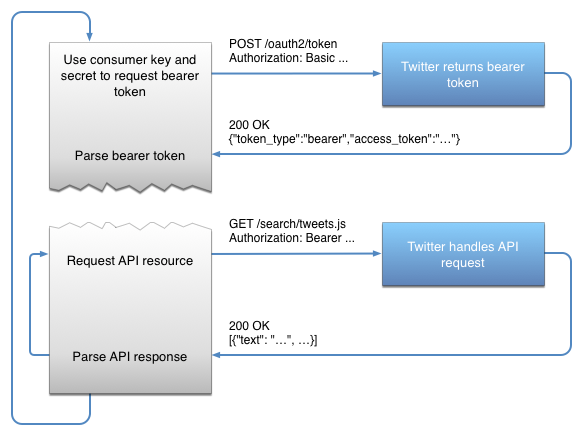
\includegraphics[width=1.00\textwidth]{C:/Users/Kvin/git/Skripsi/doc/DokumenSkripsi/Gambar/flow application-only authentication.png}
	\caption{flow application-only authentication}
	\label{fig:flow application-only authentication}
\end{figure}


\paragraph{Tentang \textit{Application-only Authentication}}
Token adalah \textit{password}. Perlu diingat bahwa \textit{consumer key} dan \textit{secret, bearer token credential}, dan \textit{the bearer token} itu sendiri memberikan akses untuk membuat permintaan atas nama aplikasi itu sendiri. Point-point ini harus dianggap sensitif layaknya \textit{password} dan tidak boleh dibagikan atau didistribusikan kepada pihak yang tidak dipercaya atau tidak berkepentingan

SSL benar-benar dibutuhkan karena ini adalah cara otentifikasi yang aman. Oleh karena itu semua \textit{request} (baik untuk mendapatkan atau menggunakan token) harus menggunakan endpoint HTTPS, yang juga merupakan syarat untuk menggunakan API v1.1.

Tidak ada konteks pengguna. Ketika mengeluarkan permintaan menggunakan \textit{application-only auth}, tidak ada konsep \textit{'current-user'}. Karena itu \textit{endpoint} seperti POST status / \textit{update} tidak akan berfungsi dengan \textit{application-only auth}.

\textit{Rate limiting}. \textit{Request} yang dibuat atas nama pengguna tidak akan menguras ketersediaan \textit{rate limit} dan \textit{request} tidak akan menguras batas penggunaan \textbf{limit} dalam \textit{user-based auth}.


\subsection{3-\textit{legged authorization}}
Cara kerja dari \textit{3-legged authorization} adalah dengan memberikan aplikasi yang anda buat untuk mengambil \textit{access token} dengan cara melakukan \textit{redirect} user dengan Twitter dan memberikan mereka sebuah otorisasi dari aplikasi yang anda buat. Cara kerja ini hampir identik dengan cara kerja yang dijelaskan pada implementasi \textit{Sign in} dengan Twitter, hanya saja terdapat dua pengecualian yaitu:

\begin{itemize}
	\item \textit{GET oauth endpoint} digunakan sebagai pengganti GET oauth
	\item User akan selalu diminta untuk mengotorisasi akses ke aplikasi anda, bahkan jika akses sebelumnya telah diberikan
\end{itemize}

Beginilah ilustrasi interaksi \textit{sign in} dengan menggunakan \textit{following flowchart}

\begin{figure}[hp]
	\centering
		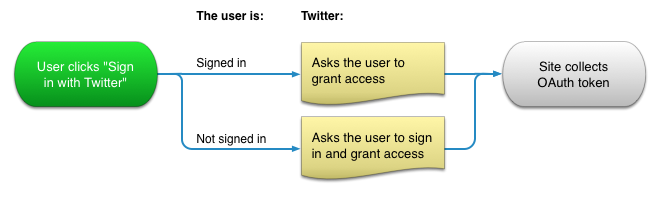
\includegraphics[width=1.00\textwidth]{C:/Users/Kvin/git/Skripsi/doc/DokumenSkripsi/Gambar/sign-in-flow3-3legged.png}
	\caption{Ilustrasi sign in}
	\label{fig:sign-in-flow3-3legged}
\end{figure}

\subsection{\textit{PIN-based authorization}}
cara kerja dari \textit{PIN-based authorization} ini ditujukan untuk aplikasi yang tidak bisa mengakses atau menanamkan \textit{web browser} untuk mengarahkan \textit{user} kepada \textit{authorization endpoint}. Contohnya adalah aplikasi yang bersifat \textit{command-line}, \textit{embedded systems}, \textit{game} konsol, dan beberapa jenis aplikasi \textit{mobile}.


Implementasi

Implementasi \textit{PIN-based authorization} ini memiliki cara kerja yang sama seperti \textit{3-legged authorization}, perbedaannya terletak pada nilai dari \textit{oauth\_callback} yang harus di set menjadi \textit{oob} saat proses pemanggilan \textit{POST oauth} atau \textit{request\_token}.

Setelah applikasi anda telah mendapatkan \textit{GET oauth/authenticate} atau \textit{GET oauth/authorize URL}, tampilkan URL kepada user agar mereka dapat menggunakan \textit{web browser} untuk mengakses Twitter.

Ketika \textit{callback oob} diminta dan user pengunjungi Twitter, \textit{user} tidak akan dipindahkan secara otomatis ke aplikasi setelah menyetujui akses. Sebaliknya, mereka akan melihat kode PIN, dengan instruksi untuk kembali ke aplikasi dan memasukkan nilai dari kode PIN tersebut.

\begin{figure}[htbp]
	\centering
		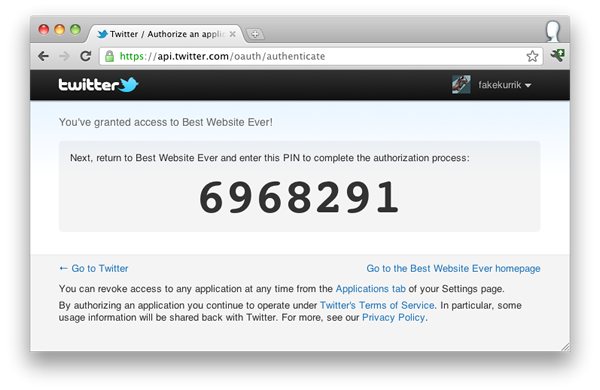
\includegraphics{C:/Users/Kvin/git/Skripsi/doc/DokumenSkripsi/Gambar/pin.png}
	\caption{Contoh PIN-based authorization}
	\label{fig:pin}
\end{figure}

Aplikasi anda harus memungkinkan \textit{user} untuk memasukkan \textit{PIN code} ini untuk menyelesaikan \textit{flow} tersebut. Nilai dari \textit{PIN code} harus lolos sebagai \textit{oauth\_verifier} untuk \textit{POST oauth/access\_token request}. Semua \textit{request} akan berjalan normal kedepannya.


%\section{KIRI}
%\label{sec:kiri}
%KIRI adalah sebuah situs atau \textit{website} yang memberi panduan tentang jalur transportasi publik. Alasan KIRI dapat berdiri adalah karenanya global warming, kemacetan, harga bensin yang semakin mahal. Ketiga alasan tersebut yang menjadi masalah sekarang ini, dan semua itu dapat diatasi dengan menaiki transportasi publik. 

%Peran dari KIRI ini adalah memberitahukan seseorang jalur transportasi publik dari satu tempat ke tempat yang dituju. Adapula format yang harus diisi dalam melakukan pencarian ini yaitu
%\begin{enumerate}
%	\item kota,
%	\item tempat awal,
%	\item tempat tujuan.
%\end{enumerate}

\section{KIRI API}
KIRI API adalah aplikasi pihak ketiga yang memungkinkan \textit{programmer} mendapatkan data tentang info jalur transportasi publik. KIRI API dapat diakses dengan beberapa cara. Semua \textit{request} harus berisikan API key, yang dapat diambil melalui KIRI API \textit{Management Dashboard}. Berikut adalah spesifikasi dari KIRI API

\begin{itemize}
	\item \textit{Routing Web Service}
	\item \textit{Search Place Web Service}
	\item \textit{Nearest Transports Web Service}
\end{itemize}

\subsection{\textit{Routing Web Service}}
\textit{Routing Web Service} adalah salah satu KIRI API yang digunakan untuk mendapatkan langkah perjalanan dari lokasi asal menuju lokasi tujuan.

Berikut ini adalah parameter \textit{request} yang diperlukan:

\begin{tabular}{ |l|l|l| }
	\hline
	\textit{Parameter} & \textit{Valid values} & \textit{Description} \\ \hline \hline
  \textit{version} & 2 & \vtop{\hbox{\strut Memberitahukan bahwa layanan yang dipakai} \hbox{\strut adalah protokol versi 2}} \\ \hline
  \textit{mode} & "\textit{findroute}" & Mengintruksikan layanan untuk mencari rute \\ \hline
  \textit{locale} & "en" or "id" & Respon bahasa yang digunakan \\ \hline
	\textit{start} & lat,lng (\textit{both are decimal values}) & Titik awal \textit{Latitude} dan \textit{longitude} \\ \hline
  \textit{finish} & lat,lng (\textit{both are decimal value}s) & Titik akhir \textit{Latitude} dan \textit{longitude}  \\ \hline
  \textit{presentation} & "\textit{mobile}" or "\textit{desktop}" & \vtop{\hbox{\strut Menentukan tipe presentasi untuk hasil keluaran.}\hbox{\strut Contoh, jika tipe presentasi "\textit{mobile}", }\hbox{\strut maka link "tel:" akan ditambahkan di hasil.}} \\ \hline
	\textit{apikey} & 16-digit \textit{hexadecimals} & API \textit{key} yang digunakan \\ \hline
\end{tabular}

\begin{lstlisting} [caption= code \textit{respond} pencarian rute]
{ 
    "status": "ok" or "error" 
    "routingresults": [ 
        {
            "steps": [
                [
                    "walk" or "none" or others,
                    "walk" or vehicle_id or "none",
                    ["lat_1,lon_1", "lan_2,lon_2", ... "lat_n,lon_n"],
                    "human readable description, dependant on locale",
                    URL for ticket booking or null (future)
                ],
                [
                    "walk" or "none" or others,
                    "walk" or vehicle_id or "none",
                    ["lat_1,lon_1", "lan_2,lon_2", ... "lat_n,lon_n"],
                    "human readable description, dependant on locale",
                    URL for ticket booking or null (future)
                ]
            ],
            "traveltime": any text string, null if and only if route is not found.
        } ,
        {
            "steps": [ ... ],
            "traveltime": "..."
        } ,
        {
            "steps": [ ... ],
            "traveltime": "..."
        } ,
        ...     
    ]
}
\end{lstlisting}

Ketika pencarian route berhasil yaitu dengan memberitahukan bahwa status "ok" seperti pada baris 2, maka server juga harus memberikan hasil dari rute, yang berisikan langkah-langkah yang disimpan di dalam array. Berikut ini adalah keterangan dari array tersebut:

\begin{itemize}
	\item \textit{Index} 0 (baris ke) berisikan "\textit{walk}" atau "\textit{none}" atau "\textit{others}". Arti dari "\textit{walk}" adalah jalan kaki, "\textit{none}" berarti rute jalan tidak ditemukan, dan "\textit{others}" berarti menggunakan kendaraan.
	\item \textit{Index} ke 1 merupakan detail dari \textit{index} ke 0 yang memiliki arti:
	\begin{itemize}
		\item Jika berisikan "\textit{walk}" berarti \textit{index} ini pun harus berisikan "\textit{walk}",
		\item Jika berisikan "\textit{none}" maka \textit{index} ini pun harus berisikan "\textit{none}",
		\item Selain itu, maka field ini berisikan id kendaraan yang dapat digunakan untuk menambilkan gambar dari id kendaraan tersebut.
	\end{itemize}
	\item \textit{Index} ke 2 berisikan \textit{array of string}, yang berisikan jalur dalam format "lat,lon". Lat adalah \textit{latitude}, dan lon adalah \textit{longitude} yaitu titik awal dan titik akhir.
	\item \textit{Index} ke 3 merupakan bentuk yang dapat dibaca oleh manusia lalu akan ditampilkan kepada pengguna. Informasi tersebut dapat berupa:
	\begin{itemize}
		\item \%\textit{fromicon} = sebuah ikon penanda yang menunjukkan titik awal atau "\textit{from}". Biasanya digunakan untuk mode presentasi perangkat bergerak.
		\item \%\textit{toicon} = sebuah ikon penanda yang menunjukkan titik akhir atau "\textit{to}". Biasanya digunakan untuk mode presentasi perangkat bergerak.
	\end{itemize}
	\item \textit{Index} ke 4 berisi URL untuk pemesanan tiket untuk travel jika tersedia. Jika tidak ada maka nilai dari \textit{index} ini bernilai null.
\end{itemize}


\subsection{\textit{Search Place Web Service}}
\textit{Search Place Web Service} berguna untuk menemukan rute perjalanan berdasarkan \textit{latitute} dan \textit{longitude} koordinat, yang tidak nyaman bagi pengguna akhir. Layanan \textit{Search Place Web Service} ini membantu untuk mengubah string teks untuk \textit{latitude} dan \textit{longitude}. Untuk permintaan \textit{routing}, berikut parameter \textit{request} yang diperlukan berikut penjelasannya:

\begin{tabular}{ |l |l |l| }
	\hline
  \textit{version} & 2 & \vtop{\hbox{\strut Memberitahukan bahwa layanan yang dipakai} \hbox{\strut adalah protokol veris 2}} \\ \hline
  \textit{mode} & "\textit{searchplace}" & mengintruksikan layanan untuk mencari tempat \\ \hline
  \textit{region} & "cgk" or "bdo" or "sub" & kota yang akan dicari tempatnya \\ \hline
	\textit{querystring} & \vtop{\hbox{\strut text apa saja dengan minimum} \hbox{\strut text satu karakter}} & \vtop{\hbox{\strut \textit{query string} yang akan dicari menggunakan}  \hbox{\strut layanan ini}} \\ \hline
	\textit{apikey} & 16-digit \textit{hexadecimals} & API \textit{key} yang digunakan \\ \hline
\end{tabular}

Berikut format kembalian dari Kiri API:
\begin{lstlisting} [caption= code \textit{respond} pencarian lokasi]
{
    "status": "ok" or "error"
    "searchresult": [
        {
            "placename": "place name"
            "location": "lat,lon"
        },
        {
            "placename": "place name"
            "location": "lat,lon"
        },
        ...
    ]
    "attributions": [
        "attribution_1", "attribution_2", ...
    ]
}
\end{lstlisting}

Ketika \textit{request find place} berhasil, server akan mengembalikan \textit{place result}, yang merupakan array dari langkah-langkah dan masing-masing berisi tentang deskripsi dalam format pemetaan:
\begin{itemize}
	\item \textit{searchresult} - berisikan array dari hasil objek:
	\begin{itemize}
		\item \textit{placename} - nama dari suatu tempat
		\item \textit{location} : \textit{latitude} dan \textit{longitude} dari suatu tempat
	\end{itemize}
	\item \textit{attributions} - berisikan \textit{array string} dan atribut tambahan yang akan ditampilkan
\end{itemize}

\subsection{\textit{Nearest Transports Web Service}}
\textit{Nearest Transports Web Service} digunakan untuk menemukan rute transportasi terdekat dengan titik yang diberikan.

Berikut parameter \textit{request} yang diperlukan berikut penjelasanya:

\begin{tabular}{ |l |l |l| }
	\hline
  \textit{version} & 2 & \vtop{\hbox{\strut Memberitahukan bahwa layanan yang dipakai} \hbox{\strut adalah protokol veris 2}} \\ \hline
  \textit{mode} & "\textit{nearbytransports}" & \vtop{\hbox{\strut mengintruksikan layanan untuk mencari rute} \hbox{\strut transportasi terdekat}} \\ \hline
  \textit{start} & \vtop{\hbox{\strut \textit{latitude} dan \textit{longitude}} \hbox{\strut (keduanya menggunakan nilai desimal)}} & kota yang akan dicari tempatnya \\ \hline
	\textit{apikey} & 16-digit \textit{hexadecimals} & API \textit{key} yang digunakan \\ \hline
\end{tabular}


Berikut format kembalian dari Kiri API:

\begin{lstlisting} [caption= code \textit{respond} menemukan lokasi terdekat]
{
    "status": "ok" or "error"
    "nearbytransports": [
        [
            "walk" or "none" or others,
            "walk" or vehicle_id or "none",
            text string,
            decimal value
        ],
        [
            "walk" or "none" or others,
            "walk" or vehicle_id or "none",
            text string,
            decimal value
        ],
        ...     
    ]
}\end{lstlisting}

Pencarian akan memberitahukan status berhasil ("\textit{ok}") atau tidak ("\textit{error}"), jika sukses maka respon akan mengembalikan array yang berisikan transportasi terdekat yang diurutkan dari yang terdeket ke yang terjauh. Berikut keterangan dari setiap array tersebut: 
\begin{itemize}
	\item \textit{Index} ke 0 dapat berisi "\textit{walk}" atau "\textit{none}" atau "\textit{others}". Artinya  jika isi dari array tersebut "\textit{walk}" berarti berjalan kaki, "\textit{none}" jika rute tidak ditemukan dan "\textit{others}" berarti menggunakan kendaran.
	\item \textit{Index} ke 1 merupakan detail dari \textit{index} 0. Artinya jika \textit{index} 0 "\textit{walk}" berarti \textit{index} 1 harus "\textit{walk}", "\textit{none}" berarti \textit{index} 1 harus "\textit{none}" dan selain itu menyatakan id kendaraan yang mana bisa dipakai untuk ditampilkan gambarnya.
	\item \textit{Index} ke 2 berisi nama kendaraan yang dapat dibaca oleh pengguna.
	\item \textit{Index} ke 3 berisi jarak dalam satuan kilometer.
\end{itemize}

\section{Twitter4J}
Twitter4J merupakan \textit{Java Library} untuk Twitter API. Dengan adanya Twitter4J ini, kita dapat dengan mudah mengintegrasikan aplikasi Java dengan Twitter \textit{service}. Twitter4J memiliki fitur-fitur sebagai berikut :

\begin{itemize}
	\item 100\% Menggunakan Bahasa Java.
	\item Tersedia untuk \textit{Android platform} dan \textit{Google App Engine}
	\item Tidak adanya dependensi, tidak memerlukan \textit{jar} tambahan.
	\item Mendukung sistem OAuth.
	\item Kompatibel dengan Twitter API 1.1
\end{itemize}

Dalam pembuatan aplikasi yang akan saya buat saya membutuhkan beberapa \textit{library} yang telah diberikan oleh Twitter4j. Berikut adalah \textit{library} yang diperlukan:
\subsection{TwitterFactory}
	
	\begin{itemize}
		\item \textit{Constant}
		
		\begin{itemize}
			\item public final class TwitterFactory
			extends java.lang.Object
			implements java.io.Serializable
			
			Sebuah \textit{factory class} untuk Twitter
		\end{itemize}
		\item \textit{Constructor}
		
		\begin{itemize}
			\item TwitterFactory()
			
			Membuat TwitterFactory dengan konfigurasi dari sumber.
			\item TwitterFactory(Configuration conf)
			
			Membuat TwitterFactory dengan konfigurasi yang diberikan.
			\item TwitterFactory(java.lang.String configTreePath)
			
			Membuat TwitterFactory yang berasal dari \textit{config tree} yang spesifik.
		\end{itemize}
		\item \textit{Methods}
		
		\begin{itemize}
			\item public Twitter getInstance()
			
			mengembalikan contoh yang terkait dengan konfigurasi.
			\item public Twitter getInstance(AccessToken accessToken)
			
			mengembalikan OAuth yang sudah diotentifikasi.
			\item public Twitter getInstance(Authorization auth)
			\item public static Twitter getSingleton()
			
			Mengembalikan \textit{singleton} standar Twitter \textit{instance}.
		\end{itemize}
	\end{itemize}
	
	
	\subsection{TwitterStream}
	\begin{itemize}
		\item \textit{Constant}
		
		\begin{itemize}
			\item public interface TwitterStream
			extends OAuthSupport, TwitterBase
			
			Sebuah \textit{factory class} untuk Twitter
		\end{itemize}
		
		\item \textit{Methods}
		
		\begin{itemize}
			\item void addConnectionLifeCycleListener(ConnectionLifeCycleListener listener)
			
			Menambahkan \textit{ConnectionLifeCycleListener}
			\item void addListener(StreamListener listener)
			
			Menambahkan listener.
			\item void removeListener(StreamListener listener)
			
			Menghilangkan listerner.
			\item void clearListeners()
			
			Menghilangkan \textit{status listener}.
			\item void replaceListener(StreamListener toBeRemoved,StreamListener toBeAdded)
			
			Menimpa listener yang sudah ada sebelumnya.
			\item void firehose(int count)
			
			Mendengarkan semua status publik.
			\item void links(int count)
			
			Mendengarkan semua status publik yang mengandung link.
			\item void retweet()
			
			Mendengarkan semua retweet.
			\item void sample()
			
			Mendengarkan status publik secara acak.
			\item void user()
			
			\textit{User Streams} menyediakan update dari semua data secara \textit{real-time}.
			\item void user(java.lang.String[] track)
			
			\textit{User Streams} menyediakan update dari semua data secara \textit{real-time}. Parameter track merupakan kata kunci untuk kata yang akan ditampilkan.
			\item StreamController site(boolean withFollowings, long[] follow)
			
			Menerima update secara \textit{real-time} untuk sejumlah pengguna tanpa perlu kerepotan dalam mengelola REST API \textit{rate limits}.
			\item void filter(FilterQuery query)
			
			Menerima status publik yang telah di \textit{filter} dari satu atau lebih kata kunci.
			\item void cleanUp()
			
			Menon-aktifkan penggunaan \textit{thread stream}.
			\item void shutdown()
			
			Menon aktifkan \textit{dispatcher thread} bersama dengan semua instansi TwitterStream.
		\end{itemize}
	\end{itemize}
	
	\subsection{TwitterStreamFactory}
	
	\begin{itemize}
		\item \textit{Constant}
		
		\begin{itemize}
			\item public final class TwitterStreamFactory
			extends java.lang.Object
			implements java.io.Serializable
			
			Sebuah \textit{factory class} untuk Twitter. Instansi dari kelas ini memiliki thread yang aman dan digunakan secara berkala lalu dapat digunakan kembali.
		\end{itemize}
		\item \textit{Constructor}
		
		\begin{itemize}
			\item TwitterStreamFactory()
			Membuat TwitterStreamFactory dengan konfigurasi dari sumber.
			\item TwitterStreamFactory(Configuration conf)
			Membuat TwitterStreamFactory dengan konfigurasi yang diberikan.
			\item TwitterStreamFactory(java.lang.String configTreePath)
			Membuat TwitterStreamFactory yang berasal dari \textit{config tree} yang spesifik.
		\end{itemize}
		\item \textit{Methods}
		
		\begin{itemize}
			\item public TwitterStream getInstance()
			
			Mengembalikan contoh yang terkait dengan konfigurasi.
			\item public TwitterStream getInstance(AccessToken accessToken)
			
			Mengembalikan OAuth yang sudah diotentifikasi.
			\item public TwitterStream getInstance(Authorization auth)
			
			Mengembalikan \textit{instance}.
			\item private TwitterStream getInstance(Configuration conf, Authorization auth)
			
			Mengembalikan \textit{instance} dengan konfigurasi dan autorisasi yang sesuai.
			\item public static Twitter getSingleton()
			
			Mengembalikan \textit{singleton} standar Twitter \textit{instance}.
		\end{itemize}
	\end{itemize}
	
	\subsection{UserStreamListener}
	\begin{itemize}
		\item \textit{Constant}
		
		\begin{itemize}
			\item public interface UserStreamListener
			extends StatusListener
		\end{itemize}
		\item \textit{Methods}
		
		\begin{itemize}
			\item void onDeletionNotice(long directMessageId, long userId)
			\item void onFriendList(long[] friendIds)
			\item void onFavorite(User source, User target, Status favoritedStatus)
			\item void onUnfavorite(User source, User target, Status unfavoritedStatus)
			\item void onFollow(User source, User followedUser)
			\item void onUnfollow(User source, User unfollowedUser)
			\item void onDirectMessage(DirectMessage directMessage)
			\item void onUserListMemberAddition(User addedMember, User listOwner, UserList list)
			\item void onUserListMemberDeletion(User deletedMember, User listOwner, UserList list)
			\item void onUserListSubscription(User subscriber, User listOwner, UserList list)
			\item void onUserListUnsubscription(User subscriber, User listOwner, UserList list)
			\item void onUserListCreation(User listOwner, UserList list)
			\item void onUserListUpdate(User listOwner, UserList list)
			\item void onUserListDeletion(User listOwner, UserList list)
			\item void onUserProfileUpdate(User updatedUser)
			\item void onBlock(User source, User blockedUser)
			\item void onUnblock(User source, User unblockedUser)
		\end{itemize}
	\end{itemize}
	
	\subsection{TweetsResources}
	\begin{itemize}
		\item \textit{Constant}
		
			\begin{itemize}
				\item public interface TweetsResources
			\end{itemize}
		\item \textit{Methods}
		
		\begin{itemize}
			\item ResponseList<Status> getRetweets(long statusId) throws TwitterException
			
			Mengembalikan sampai dengan 100 retweet pertama yang diberikan.
			\item IDs getRetweeterIds(long statusId, long cursor) throws TwitterException
			
			Mengembalikan sampai dengan 100 ID pengguna yang telah melakukan retweet oleh parameter ID tertentu
			\item IDs getRetweeterIds(long statusId, int count, long cursor) throws TwitterException
			
			Mengembalikan sampai dengan "\textit{count}" ID pengguna yang telah melakukan retweet oleh parameter ID tertentu
			\item Status showStatus(long id) throws TwitterException
			
			Mengembalikan \textit{single status} yang ditentukan oleh parameter ID yang telah ditentukan.
			\item Status destroyStatus(long statusId) throws TwitterException
			
			Menghapus status yang ditentukan oleh parameter ID yang telah ditentukan.
			\item Status updateStatus(java.lang.String status) throws TwitterException
			
			Melakukan update status oleh user yang telah diotentifikasi
			\item Status updateStatus(StatusUpdate latestStatus) throws TwitterException
			
			Melakukan update status oleh user yang telah diotentifikasi.
			\item Status retweetStatus(long statusId) throws TwitterException
			
			Melakukan retweet.
			\item OEmbed getOEmbed(OEmbedRequest req) throws TwitterException
			Mengembalikan informasi yang dapat merepresentasikan \textit{third party} Tweet
			
			\item ResponseList<Status> lookup(long[] ids) throws TwitterException
			
			Mengembalikan \textit{fully-hydrated tweet objects} sampai dengan 100 tweet setiap \textit{request}nya.
			\item UploadedMedia uploadMedia(java.io.File mediaFile) throws TwitterException
			
			Melakukan \textit{upload} media gambar yang telah di dilampirkan via updateStatus(twitter4j.StatusUpdate)
		\end{itemize}
	\end{itemize}

	\subsection{OAuthSupport}
	\begin{itemize}
		\item \textit{Constant}
		
			\begin{itemize}
				\item public interface OAuthSupport
			\end{itemize}
		\item \textit{Methods}
		
		\begin{itemize}
			\item void setOAuthConsumer(java.lang.String consumerKey, java.lang.String consumerSecret)
			
			Melakukan pengaturan terhadap \textit{consumer key} dan \textit{consumer secret }.
			\item RequestToken getOAuthRequestToken() throws TwitterException
			
			Mengambil \textit{request token}.
			\item RequestToken getOAuthRequestToken(java.lang.String callbackURL) throws TwitterException
			
			
			Mengambil \textit{request token}.
			\item RequestToken getOAuthRequestToken(java.lang.String callbackURL, java.lang.String xAuthAccessType) throws TwitterException
			
			Mengambil \textit{request token}.
			\item AccessToken getOAuthAccessToken() throws TwitterException
			
			Mengembalikan \textit{access token} yang terkait dengan instansi ini. Jika tidak ada instansi pada \textit{access token} maka akan mengambil \textit{access token} yang baru.
			\item AccessToken getOAuthAccessToken(java.lang.String oauthVerifier) throws TwitterException
			
			Mengambil \textit{request token}.
			\item AccessToken getOAuthAccessToken(RequestToken requestToken) throws TwitterException
			
			Mengambil \textit{access token} yang terkait dengan \textit{request token }dan \textit{userId} yang telah diberikan
			\item AccessToken getOAuthAccessToken(RequestToken requestToken, java.lang.String oauthVerifier) throws TwitterException
			
			Mengambil \textit{access token} yang terkait dengan \textit{request token }dan \textit{userId} yang telah diberikan
			\item AccessToken getOAuthAccessToken(java.lang.String screenName, java.lang.String password) throws TwitterException
			
			Mengambil \textit{access token} yang terkait dengan \textit{screen name}dan \textit{password} yang telah diberikan
			\item void setOAuthAccessToken(AccessToken accessToken)
			
			Melakukan pengaturan pada \textit{access token}
		\end{itemize}
	\end{itemize}

\subsection{RequestToken}
	\begin{itemize}
		\item \textit{Constant}
		
		\begin{itemize}
			\item public final class RequestToken
			extends OAuthToken
			implements java.io.Serializable
			
		\end{itemize}
		\item \textit{Constructor}
		
		\begin{itemize}
			\item RequestToken(HttpResponse res, OAuthSupport oauth) 
			\item RequestToken(java.lang.String token, java.lang.String tokenSecret)
			\item RequestToken(java.lang.String token, java.lang.String tokenSecret, OAuthSupport oauth) 
		\end{itemize}
		\item \textit{Methods}
		
		\begin{itemize}
			\item public java.lang.String getAuthorizationURL()
			\item public java.lang.String getAuthenticationURL()
		\end{itemize}
	\end{itemize}
	
\subsection{AccessToken}
	\begin{itemize}
		\item \textit{Constant}
		
		\begin{itemize}
			\item public class AccessToken
			extends OAuthToken
			implements java.io.Serializable
						
		\end{itemize}
		\item \textit{Constructor}
		
		\begin{itemize}
			\item AccessToken(HttpResponse res) 
			\item AccessToken(java.lang.String token, java.lang.String tokenSecret) 
			\item AccessToken(java.lang.String token, java.lang.String tokenSecret, long userId) 
		\end{itemize}
		\item \textit{Methods}
		
		\begin{itemize}
			\item public java.lang.String getScreenName()
			
			Mengembalikan \textit{screen name}
			\item public long getUserId()
			
			Mengembalikan \textit{user id}
			\item public boolean equals(java.lang.Object o)
			\item public int hashCode()
			\item public java.lang.String toString()
		\end{itemize}
	\end{itemize}
	
	\subsection{Status}
	\begin{itemize}
		\item \textit{Constant}
		
		\begin{itemize}
			\item public interface Status
			extends java.lang.Comparable<Status>, TwitterResponse, EntitySupport, java.io.Serializable
						
		\end{itemize}
		\item \textit{Methods}
		
		\begin{itemize}
			\item java.util.Date getCreatedAts()
			
			Mengembalikan \textit{created\_at}
			\item public long getUserId()
			
			Mengembalikan \textit{user id}
			\item java.lang.String getText()
			
			Mengembalikan teks dari status
			\item java.lang.String getSource()
			
			Mengembalikan \textit{source}
			\item boolean isTruncated()
			
			Menguji apakah sebuah status terpotong atau tidak
			\item long getInReplyToStatusId()
			
			Mengembalikan \textit{in\_reply\_tostatus\_id}
			\item long getInReplyToUserId()
			
			Mengembalikan \textit{in\_reply\_user\_id}
			\item java.lang.String getInReplyToScreenName()
			
			Mengembalikan \textit{in\_reply\_to\_screen\_name}
			\item GeoLocation getGeoLocation()
			
			Mengembalikan lokasi dari suatu \textit{tweet} jika tersedia.
			\item Place getPlace()
			
			Mengembalikan tempat yang terdapat pada sebuah status.
			\item boolean isFavorited()
			
			Menguji apakah status tersebut \textit{favorite} atau tidak
			\item boolean isRetweeted()
			
			Menguji apakah status tersebut \textit{retweet} atau tidak
			\item int getFavoriteCount()
			
			Menunjukkan berapa kali Tweet telah menjadi \textit{favorite}
			\item User getUser()
			
			Mengembalikan \textit{user} yang terdapat pada sebuah status.
			\item boolean isRetweet()
			\item Status getRetweetedStatus()
			\item long[] getContributors()
			
			Mengembalikan array yang berisi kontributor atau mengembalikan \textit{null} jika tidak ada kontributor yang terkait dengan status ini
			\item int getRetweetCount()
			
			Menunjukkan berapa kali Tweet telah di \textit{retweet}, jika belum terdapat maka akan mengembalikan nilai -1
			\item boolean isRetweetedByMe()
			
			Mengembalikan nilai \textit{true} jika \textit{user} yang telah diotentifikasi melakukan \textit{retweet} terhadap suatu \textit{tweet}, atau mengembalikan nilai \textit{false} jika tidak.
			\item long getCurrentUserRetweetId()
			
			Mengembalikan \textit{retweet id} sebuah \textit{tweet} dari \textit{user} yang telah diotentifikasi, jika belum terdapat maka akan mengembalikan nilai -1L
			\item boolean isPossiblySensitive()
			
			Mengembalikan nilai \textit{true} jika pada status terdapat \textit{sensitive links}
			\item java.lang.String getLang()
			
			Mengembalikan \textit{lang} dari sebuah status teks jika tersedia
			\item Scopes getScopes()
			
			Mengembalikan target dari \textit{scopes} yang diaplikasikan kepada sebuah status.
		\end{itemize}
	\end{itemize}
	
	\subsection{TweetsResources}
	\begin{itemize}
		\item \textit{Constant}
		
		\begin{itemize}
			\item public interface TweetsResources
						
		\end{itemize}
		\item \textit{Methods}
		
		\begin{itemize}
			\item ResponseList<Status> getRetweets(long statusId) throws TwitterException
			
			Mengembalikan hingga dengan seratus \textit{retweet} pertama
			\item IDs getRetweeterIds(long statusId, long cursor) throws TwitterException
			
			Mengembalikan hingga dengan 100 \textit{user ID} yang melakukan \textit{retweet} terhadap \textit{tweet} ditentukan dari \textit{id parameter}
			\item IDs getRetweeterIds(long statusId, int count, long cursor) throws TwitterException
			
			Mengembalikan hingga dengan \textit{"count"} \textit{user ID} yang melakukan \textit{retweet} terhadap \textit{tweet} ditentukan dari \textit{id parameter}
			\item Status showStatus(long id) throws TwitterException
			
			Mengembalikan \textit{status} yang ditentukan dari parameter id.
			\item Status destroyStatus(long statusId) throws TwitterException
			
			Menghapus \textit{status} yang ditentukan dari parameter id.
			\item Status updateStatus(java.lang.String status) throws TwitterException
			
			Melakukan \textit{update status} terhadap \textit{user} yang telah diotentifikasi.
			\item Status updateStatus(StatusUpdate latestStatus) throws TwitterException
			
			Melakukan \textit{update status} terhadap \textit{user} yang telah diotentifikasi.
			\item Status retweetStatus(long statusId) throws TwitterException
			
			Melakukan \textit{retweet} terhadap sebuah \textit{tweet}.
			\item OEmbed getOEmbed(OEmbedRequest req) throws TwitterException
			
			Mengembalikan informasi yang mengizinkan terciptanya \textit{embedded representation} dari tweet yang berada di \textit{third party sites}
			\item ResponseList<Status> lookup(long[] ids) throws TwitterException
			
			Mengembalikan objek \textit{tweet} hingga dengan 100 \textit{tweet} per \textbf{request}.
			\item UploadedMedia uploadMedia(java.io.File mediaFile) throws TwitterException
			
			Melakukan \textit{upload} gambar.
		\end{itemize}
	\end{itemize}
%\subsection{Contoh Kode}
%Untuk menjalankan ini semua, anda harus mempunyai OAuth credential yang telah dikonfigurasi pada twitter4j.properties.

%\begin{itemize}
%	\item Melakukan Tweet
	
%	Anda dapat melakukan Tweet seperti "Selamat pagi" dengan menggunakan \textit{method} Twitter.updateStatus().
%	\begin{lstlisting} [caption= code untuk melakukan Tweet]
%	{
%			Twitter twitter = TwitterFactory.getSingleton();
%			Status status = twitter.updateStatus(latestStatus);
%			System.out.println("Successfully updated the status to [" + status.getText() + "].");
%	}\end{lstlisting}
%	\item Mendapatkan Timeline
%	
%	Berikut adalah contoh kode untuk mendapatkan \textit{timeline}
%	\begin{lstlisting} [caption= code untuk mendapatkan \textit{timeline}]
%	{
%			Twitter twitter = TwitterFactory.getSingleton();
%    List<Status> statuses = twitter.getHomeTimeline();
%    System.out.println("Showing home timeline.");
%    for (Status status : statuses) {
%        System.out.println(status.getUser().getName() + ":" +
%                           status.getText());
%    }
%	}\end{lstlisting}
%	\item Mengirim dan Menerima \textit{Direct Message}
%	
%	Anda dapat mengirim dan menerima \textit{direct message} dengan menggunakan \textit{method} Twitter.sendDirectMessage() atau Twitter.getDirectMessages(). Berikut adalah contoh kodenya.
%	\begin{lstlisting} [caption= code untuk mengirim \textit{direct message}]
%	{
%			 Twitter sender = TwitterFactory.getSingleton();
%    DirectMessage message = sender.sendDirectMessage(recipientId, message);
%    System.out.println("Sent: " message.getText() + " to @" + message.getRecipientScreenName());
%    }
%	}\end{lstlisting}
%	\item Mencari Tweet
%	
%	Mencari Tweet dapat dilakukan dengan menggunakan kelas \textit{query} atau dengan menggunakan method Twitter.seach(twitter4j.Query). Berikut adalah contoh kodenya
%	\begin{lstlisting} [caption= code untuk mencari Tweet]
%	{
%			 Twitter twitter = TwitterFactory.getSingleton();
%    Query query = new Query("source:twitter4j yusukey");
%    QueryResult result = twitter.search(query);
%    for (Status status : result.getTweets()) {
%        System.out.println("@" + status.getUser().getScreenName() + ":" + status.getText());
%    }
%    }
%	}\end{lstlisting}
%	\item OAuth support
%	
%	Dengan menggunakan skema OAuth authorization, sebuah aplikasi dapat mengakses akun user tanpa menggunakan userid dan password. Anda hanya perlu melakukan registrasi %pada aplikasi anda ke http://twitter.com/oauth\_clients/new untuk mendapatkan \textit{consumer key}, dan \textit{consumer secret } terlebih dahulu. \textit{Key / %secret pair} dapat di set menggunakan Twitter\#setOAuthConsumer() atau mengikuti petunjuk \textit{system properties}:
%	\begin{itemize}
%		\item Dtwitter4j.oauth.consumerKey=[consumer key]
%%		\item Dtwitter4j.oauth.consumerSecret=[consumer secret]
%	\end{itemize}
%	Anda tidak perlu memiliki izin untuk mengakses sebuah akun tetapi harus memiliki \textit{access token} dengan mengarahkan user ke URL \textit{authorization} sebagai %berikut:
%	\begin{lstlisting} [caption= code untuk mengarahkan user ke URL \textit{authorization}]
%	{
%			 public static void main(String args[]) throws Exception{
%    // The factory instance is re-useable and thread safe.
%    Twitter twitter = TwitterFactory.getSingleton();
%    twitter.setOAuthConsumer("[consumer key]", "[consumer secret]");
%    RequestToken requestToken = twitter.getOAuthRequestToken();
%    AccessToken accessToken = null;
%    BufferedReader br = new BufferedReader(new InputStreamReader(System.in));
%    while (null == accessToken) {
%      System.out.println("Open the following URL and grant access to your account:");
%      System.out.println(requestToken.getAuthorizationURL());
%      System.out.print("Enter the PIN(if aviailable) or just hit enter.[PIN]:");
%      String pin = br.readLine();
%      try{
%         if(pin.length() > 0){
%           accessToken = twitter.getOAuthAccessToken(requestToken, pin);
%         }else{
%           accessToken = twitter.getOAuthAccessToken();
%         }
%      } catch (TwitterException te) {
%        if(401 == te.getStatusCode()){
%          System.out.println("Unable to get the access token.");
%        }else{
%          te.printStackTrace();
%        }
%      }
%    }
%    //persist to the accessToken for future reference.
%    storeAccessToken(twitter.verifyCredentials().getId() , accessToken);
%    Status status = twitter.updateStatus(args[0]);
%    System.out.println("Successfully updated the status to [" + status.getText() + "].");
%    System.exit(0);
%  }
%  private static void storeAccessToken(int useId, AccessToken accessToken){
%    //store accessToken.getToken()
%    //store accessToken.getTokenSecret()
%  }
%    }
%	\end{lstlisting}
%	Setelah mendapatkan \textit{Access Token}, maka \textit{Request Token} sudah tidak berlaku lagi. Anda dapat menggunakan Access Token untuk sistem \textit{file} dengan melakukan seriliasi objek, atau dengan mendapatkan token dan secret dari AccesToken\#getToken() dan AccessToken\#getTokenSecret().
%	\begin{lstlisting} [caption= code untuk mmendapatkan \textit{token} dan \textit{tokenSecret}]
%	{
%		public static void main(String args[]) throws Exception{
%			// The factory instance is re-useable and thread safe.
%			TwitterFactory factory = new TwitterFactory();
%			AccessToken accessToken = loadAccessToken(Integer.parseInt(args[0]));
%			Twitter twitter = factory.getInstance);
%			twitter.setOAuthConsumerKey("[consumer key]", "[consumer secret]");
%			twitter.setOAuthAccessToken(accessToken);
%			Status status = twitter.updateStatus(args[1]);
%			System.out.println("Successfully updated the status to [" + status.getText() + "].");
%			System.exit(0);
%		}
%		private static AccessToken loadAccessToken(int useId){
%			String token = // load from a persistent store
%			String tokenSecret = // load from a persistent store
%			return new AccessToken(token, tokenSecret);
%		}
%  }
%	\end{lstlisting}
	
%	\item \textit{Streaming API}
%	\textit{TwitterStream class} memiliki beberapa method yang telah disiapkan untuk \textit{Streaming API}. Yang anda perlukan hanya mengimplementasikan \textit{StatusListener}. Berikut adalah contoh kodenya:
%	\begin{lstlisting} [caption= contoh code untuk Streaming API]
%	{
%		public static void main(String[] args) throws TwitterException, IOException{
%			StatusListener listener = new StatusListener(){
%					public void onStatus(Status status) {
%							System.out.println(status.getUser().getName() + " : " + status.getText());
%					}
%					public void onDeletionNotice(StatusDeletionNotice statusDeletionNotice) {}
%					public void onTrackLimitationNotice(int numberOfLimitedStatuses) {}
%					public void onException(Exception ex) {
%							ex.printStackTrace();
%					}
%			};
%			TwitterStream twitterStream = new TwitterStreamFactory().getInstance();
%			twitterStream.addListener(listener);
%			// sample() method internally creates a thread which manipulates TwitterStream and calls these adequate listener methods continuously.
%			twitterStream.sample();
%		}
%  }
%	\end{lstlisting}
%\end{itemize}